\documentclass{article}
\usepackage{eecstex}

\newcommand{\E}{\mathbb{E}}

\title{CS 70 HW 13}
\author{Bryan Ngo}
\date{2020-11-26}

\begin{document}

\maketitle

\section{Random Cuckoo Hashing}

\subsection{}

The probability of no collisions when hashing \(\Pr(d_1) = 1\) trivially.
When hashing \(d_2\), \(\Pr(d_2) = \frac{n - 1}{n}\).
Inductively,
\begin{align}
    \Pr(d_n) &= \prod_{i \in [1, n]} \frac{n - i + 1}{n} = \frac{n!}{n^n} \\
    \lim_{n \to \infty} \frac{n!}{n^n} &= 0
\end{align}

\subsection{}

We can model this problem as a geometric distribution with parameter \(\frac{1}{n}\).
Let our random variable \(X\) be the number of attempts.
Thus, we have
\begin{equation}
    \E(X) = \frac{1}{p} = n
\end{equation}
However, we must subtract one because the last hashing attempt will be successful, so \(\E(C) = \E(X) - 1 = n - 1\).

\subsection{}

We can use the same distribution, except we have parameter \(p = \frac{n - k + 1}{n}\).
This means \(\E(C_k) = \frac{n}{n - k + 1} - 1 = \frac{k - 1}{n - k + 1}\).

\subsection{}

By linearity of expectation, we can construct a sum
\begin{equation}
    \E(C) = \sum_{i \in [1, n]} \frac{i - 1}{n - i + 1}
\end{equation}

\newpage
\section{Geometric and Poisson}

\begin{lemma}
    For a geometric distribution with random variable \(X\) and parameter \(p\),
    \begin{equation}
        \Pr(X > i) = (1 - p)^i
    \end{equation}
\end{lemma}
\begin{proof}
    \begin{align}
        \Pr(X > i) &= \Pr(X \geqslant i) - \Pr(X = i) \\
        &= (1 - p)^{i - 1} - (1 - p)^{i - 1} p \\
        &= (1 - p)^{i - 1} (1 - p) = (1 - p)^i
    \end{align}
\end{proof}
Finding \(\Pr(X > Y)\),
\begin{align}
    \Pr(X > Y) &= \sum_{i \geqslant 0} \Pr(Y = i, X > i) \\
    &= \sum_{i \geqslant 0} \Pr(Y = i) \Pr(X > i) \\
    &= \sum_{i \geqslant 0} \frac{\lambda^i}{i!} e^{-\lambda} (1 - p)^i \\
    &= e^{-\lambda} \sum_{i \geqslant 0} \frac{(\lambda (1 - p))^i}{i!} \\
    &= e^{-\lambda} e^{\lambda (1 - p)} = e^{-\lambda p}
\end{align}

\section{Exploring the Geometric Distribution}

\begin{align}
    \Pr(X = i) &= (1 - p)^{i - 1} p \\
    \Pr(Y = i) &= (1 - q)^{i - 1} q
\end{align}
The distribution of \(\min\{X, Y\}\) for two geometric distributions by inclusion-exclusion is
\begin{align}
    \Pr(\min\{X, Y\} = i) &= \Pr(X = i, Y \geqslant i) + \Pr(Y = i, X \geqslant i) - \Pr(X = i, Y = i) \\
    &= \Pr(X = i) \Pr(Y \geqslant i) + \Pr(Y = i) \Pr(X \geqslant i) - \Pr(X = i) \Pr(Y = i) \\
    &= (1 - p)^{i - 1} p (1 - q)^{i - 1} + (1 - q)^{i - 1} q (1 - p)^{i - 1} - ((1 - p) (1 - q))^{i - 1} pq \\
    &= ((1 - p) (1 - q))^{i - 1} p + ((1 - p) (1 - q))^{i - 1} q - ((1 - p) (1 - q))^{i - 1} pq \\
    &= ((1 - p) (1 - q))^{i - 1} (p + q - pq)
\end{align}
which is a geometric distribution with parameter \(p + q - pq\).

\newpage
\section{Lunch Meeting}

The probability of both Alice and Bob follow a uniform distribution.
So the probability of both Alice and Bob meeting appear like this:
\begin{center}
    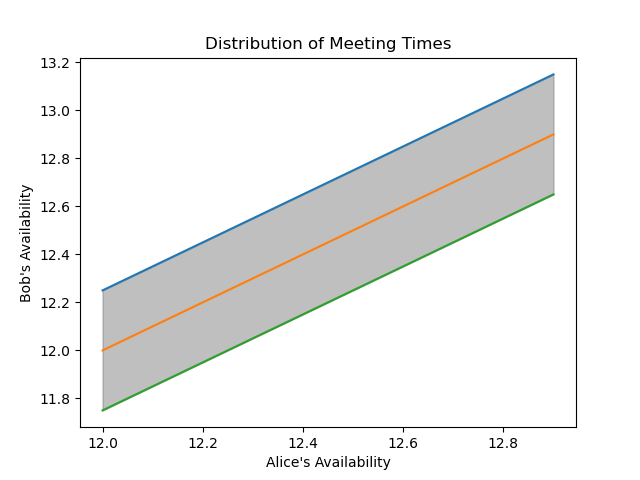
\includegraphics[width=0.8\textwidth]{q4.png}
\end{center}
Thus, \(\Pr(A = i, B = i)\) is nothing more than the area of the parallelogram bounded by the unit square, or \(\Pr(A = i, B = i) = 0.5 \cdot 1 - 0.25^2 = \num{0.4375}\).

\section{Sundry}

I worked on this homework by myself.

\end{document}
